\chapter{Working}
 
 	\begin{figure}[ht]
 	\centering
	 	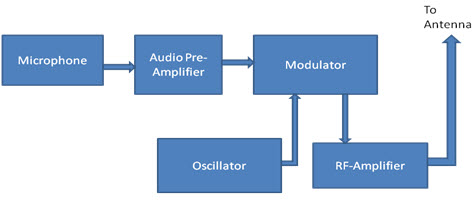
\includegraphics[width=0.70\textwidth]{blockdiag.jpg}
 	\caption{FM transmitter circuit block diagram}
 	\label{fig:block}
 \end{figure}
 \section{Pre-amplification stage}
	\begin{itemize}
		
%		\item The first stage is a preamplifier stage based on transistor Q1
%		\item Collector based amplifier stage where resistor R2 sets the collector current
%		and R1 provided the necessary collector to base bias.
%		\item  C1 is the input DC decoupling
%		capacitor which couples the input audio signal to the Q1 base. 
%		\item C8 is the power supply bypass capacitor.
	\item The first stage of the circuit is a preamplifier stage based on transistor Q1 which can be any low noise npn transistor. 
	\item This is a collector to base biased amplifier stage where resistor R2 sets the collector current and R1 provided the necessary collector to base bias.
	\item C1 is the input DC decoupling capacitor which couples the input audio signal to the Q1 base.
	\item C8 is the power supply bypass capacitor.
	\item If you are going with a battery eliminator, then it must be well filtered and regulated. C3 and C4 are for suppressing the ripple if any.
	\item C3 prevents any noise disturbance to pass into the input of transistor \item Q2 and C4 suppresses voltage spikes and noise disturbance in the power supply.	
	\end{itemize} 		
%
 \section{Modulator \& Oscillator stage}
 	\begin{itemize}
 \item Next stage is the oscillator cum modulator stage.
 \item Modulation stage is served by transistor Q2. Q2 can be
 	2N2369, 2N2219, 2N1711. 
 	\item Electrolytic capacitor C2 couples the output of the first stage to the second stage. 
 	\item R3 and R4 are the biasing resistors of Q2. 
 	\item R5 is the emitter resistor of Q2. 
 	\item Inductor L1 and trimmer capacitor C5 form the tank circuit which is necessary for creating oscillations. \item The modulated FM signal is available at the collector of Q2 and it is coupled to the antenna using capacitor C9.
 	\item L1 can be constructed by making 4 turns of 1mm enamelled copper wire on a 10mm diameter plastic former.
 	\item Trimmer C5 can be used for adjusting the transmission frequency.
 	\item Trimmer capacitor C6 can be adjusted for obtaining the maximum range.
 	\item The antenna can be a 1m copper wire.
 		\end{itemize} 
%		\begin{itemize}
%	
%	\item Oscillator cum modulator stage
%	\item Capacitor C2 couples the output of the first stage to the second stage.
%	\item R3 and R4 are the biasing resistors of Q2.
%	\item R5 is the emitter resistance of Q2. 
%	\item Inductors	L1 and trimmer capacitor C5 form the tank circuit which creates the
%	oscillations. 
%	\item The modulated FM signal is available at the collector of Q2 and is coupled
%	to the antenna using capacitor C9.
%	
%\end{itemize}